\section{Use cases}

\subsection{TaskDo}

TaskDo \citep{taskdo} is a task manager application written using CoffeeScript \citep{coffeescript}, Spine \citep{spinejs} and Atmosphere. It features offline usage, synchronization with Google Tasks API \citep{google_tasks} and is bundled as application for Mac platform using MacGap. \citep{macgap}

The strong point of TaskDo is its close resemblance to native application. TaskDo is bundled as one and it is highly responsive. This responsiveness is achieved by storing objects locally and synchronizing them with Google Tasks API using Atmosphere.

\begin{figure}[htbp]
  \centering
    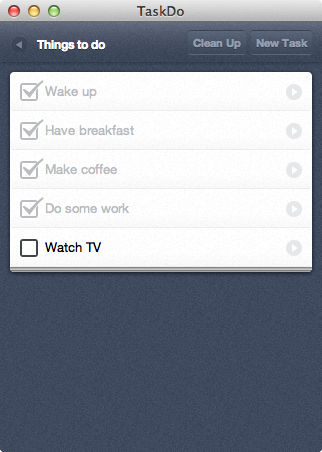
\includegraphics[height=3in]{TaskDo.png}
  \caption{Screenshot of TaskDo}
  \label{fig:taskdo}
\end{figure}

One of the problems during implementation was OAuth authentication. To successfully authenticate user, the OAuth2 protocol \citep{oauth} first requires redirection to provider's website. Then the user has to confirm that they want to share their data with third party application. At the end of the authentication process the user is redirected back to the original application.

\begin{figure}[ht!]
  \centering
    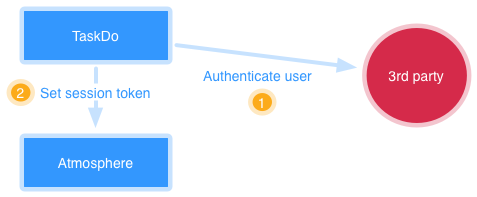
\includegraphics[width=3.5in]{TaskDoDiagram.png}
  \caption{Diagram of OAuth authentication}
  \label{fig:taskdo_diagram}
\end{figure}

Now the application is sent a session token, which has to be used with every subsequent API call in form of HTTP header.

Atmosphere provides a method for sending custom HTTP header with each request. TaskDo implements logic for completing the authentication process and then updates configuration for resource client to use the newly retrieved token with each request.

The Google Tasks API also returns JSON in a slightly more complicated format. For this reason, Atmosphere allows configuration of the way data are extracted from the response.

\subsection{Edukit}
\label{sec:edukit}

% \begin{figure}[htbp]
%   \centering
%     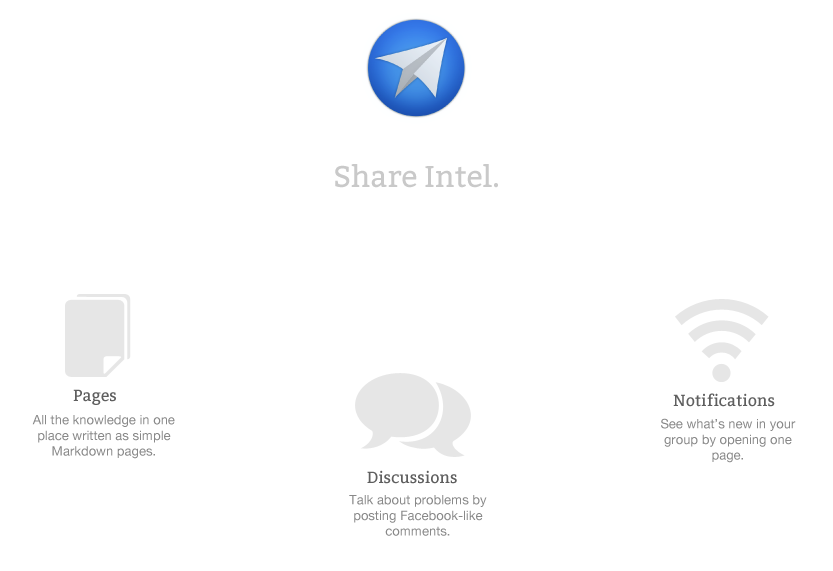
\includegraphics[height=3in]{Edukit.png}
%   \caption{The marketing diagram describing Edukit}
%   \label{fig:figures_Edukit}
% \end{figure}

Edukit is a data sharing platform intended for students. It features simple wiki-like pages, discussions and notifications. It helps students share and discuss knowledge.

Edukit is an existing web application written in Ruby on Rails, not using Atmosphere. Edukit Beta is the new version that is written in JavaScript and uses Atmosphere to communicate with the API of the existing version.

One of its key strengths is ease of use, the social aspect and the speed. Edukit is a very fast web application because of its minimal nature. But generating a new page with each action and delivering it to user can only be so fast. By using Atmosphere in Edukit Beta it was possible to go even further and make the application feel like a desktop application that provides instant response to almost every action made by user.

\begin{figure}[htbp]
  \centering
    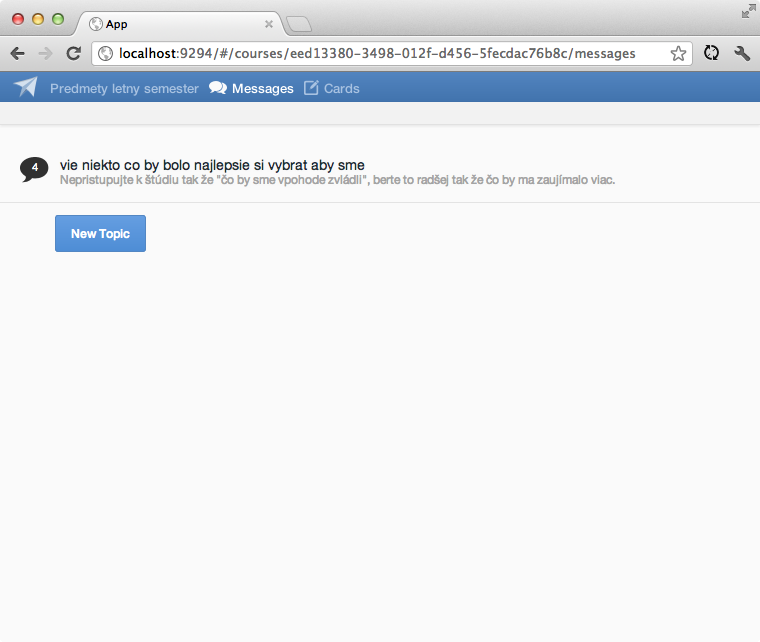
\includegraphics[height=3in]{EdukitScreen.png}
  \caption{Screenshot of Edukit showing list of topics in a course}
  \label{fig:figures_EdukitScreen}
\end{figure}

The new version of Edukit uses Spine.js and Atmosphere to create fully client-side web application, which stores data locally into the local storage of browser.

Atmosphere synchronizes these local data with the REST API of the original Edukit in the background. There are no changes in the original application involved, only exposing the REST API. The result is that it is possible to use both applications, the old and the new one at the same time.

\subsubsection{Real-time updates}

Edukit also utilizes the real-time notification server provided by Atmosphere as pictured in Figure \ref{fig:figures_EdukitMessages}. When a user creates a new message, a request is made against the original API written in Ruby. \raisebox{-2.5mm}{
\includegraphics[height=0.3in]{Item1.png}} The Ruby application collects information about the newly created message: its sender, contents and intended recipients. (All users that are in the course.) This information is then sent to Atmosphere notification server. \raisebox{-2.5mm}{
\includegraphics[height=0.3in]{Item2.png}} Atmosphere server now forwards the notification to clients connected via WebSocket. \raisebox{-2.5mm}{
\includegraphics[height=0.3in]{Item3.png}}

\begin{figure}[htbp]
  \centering
    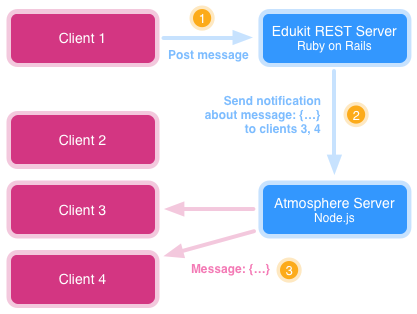
\includegraphics[height=2.5in]{figures/EdukitMessages.png}
  \caption{Posting messages with real-time updates in Edukit}
  \label{fig:figures_EdukitMessages}
\end{figure}


Since the Ruby application and the live notification server are running on the same machine, and the Atmosphere server is written in Node.js, there is almost no extra processing time for the original request. Thanks to non-blocking event-based API of Node.js, it is possible to allow access for many users at once without using multithreading. \citep{nodejs_book} The result is ability to chat in real time with other users who are currently viewing the same topic.

\subsubsection{Failure recovery by using UUIDs}

Edukit implements failure recovery (see section \ref{sec:failure_recovery}) by using same object identifiers on both client and server side.

When a local object is created, it is assigned a new UUID. When it is synchronized, the server creates it in the database, and sets it is identifier to the one created on the client side.

This helps prevent the case of one local object being created two times on the server side in case of network failure. This situation can never happen, because server uses client identifier to create remote object, so if an object with same identifier already exists, it will simply return that object instead of creating a new one.

\subsection{Zone}

Zone is an application for Mac that allows simple time tracking. At its first iteration the mission was to help people focus on their work by ``zoning in'', \citep{zone_app} which would make the toolbar icon purple, reminding user they are working.

At later iterations, a new feature was added: Overview of previous zones throughout the week. This feature would help users find their productive time of the day by letting them visualize how long they were able to focus without taking a break.

The last iteration added synchronization with a web service. Its web interface allows viewing zones, exporting them into PDF and generating invoices. The last iteration utilizes Atmosphere's Cocoa client library to synchronize local data about zones with the web interface.

\begin{figure}[htbp]
  \centering
    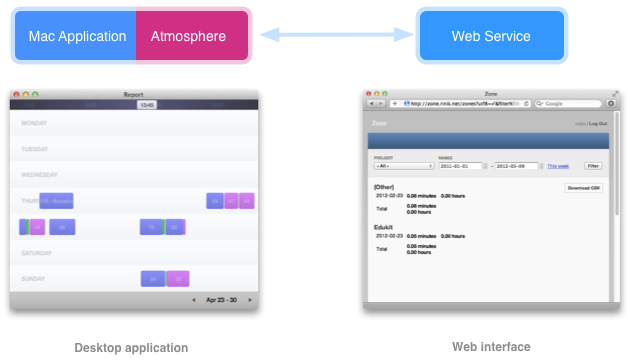
\includegraphics[height=2.5in]{figures/ZoneDiagram.png}
  \caption{Components of Zone}
  \label{fig:figures_ZoneDiagram}
\end{figure}